\documentclass{article}
\usepackage[utf8]{inputenc}
\usepackage{graphicx}
\usepackage{neuralnetwork}
%\usepackage[margin=2in]{geometry}



\title{Neural Networks: Mathematics of Backpropagation}
\author{Sylesh Suresh and Nikhil Sardana}
\date{October 2017}

\begin{document}

\maketitle

\section{Introduction}
Recall our network from the previous lecture:

Through forward propagation, we calculated our prediction $x_2$ for the input $x_0$. Keep in mind, however, that this prediction is essentially a stab in the dark. We multiplied the input by randomly initialized weights and randomly initialized biases through each layer and calculated an output. At this stage, the output is simply a random guess and is probably very different from the target/true output $y$. In order to make our neural network more accurate, we must change the weights and biases so that our predicted output $x_2$ gets as close to the target output $y$ as possible.

To accomplish this, we will use backpropagation. The first step is to quantify exactly how wrong our prediction is; in other words, we will use an error function. We define the error function as \[E = \frac{1}{2}||x_2-y||^2\]
This makes sense; $E$ increases as the difference between $x_2$ and $y$ increases. The goal of backpropagation is to minimize this error, which will get $x_2$ and $y$ as close together as possible, making $x_2$ a better prediction.

To minimize $E$, we must change the weights and biases accordingly. Unfortunately, there are many weights and biases (just look at the diagram above), so we can’t just test many different combinations weights and biases and see which one yields the least error. That said, we can use differentiation to help us. By taking the partial derivative of the error with respect to a particular weight, we will know how to change the weight in order to decrease the error; changing the weight in the direction of the negative partial derivative will decrease the error. Please see the "Neural Networks: Part 2", Sections 4.1-4.3, for a more in-depth explanation as to why calculating the partial derivatives helps us minimize the error function.


\section{Non-Vectorized Backpropagation}
We've already covered how to backpropagate in the vectorized form (Neural Networks: Part 2, Section 4.5). However, this can be confusing to many students, particularly the parts with matrix transformations and Hadamard products. To alleviate any confusion, let's walk through backpropagation without any vectors at all.

\subsection{Defining the Network}
Consider the following neural network:

\begin{center}
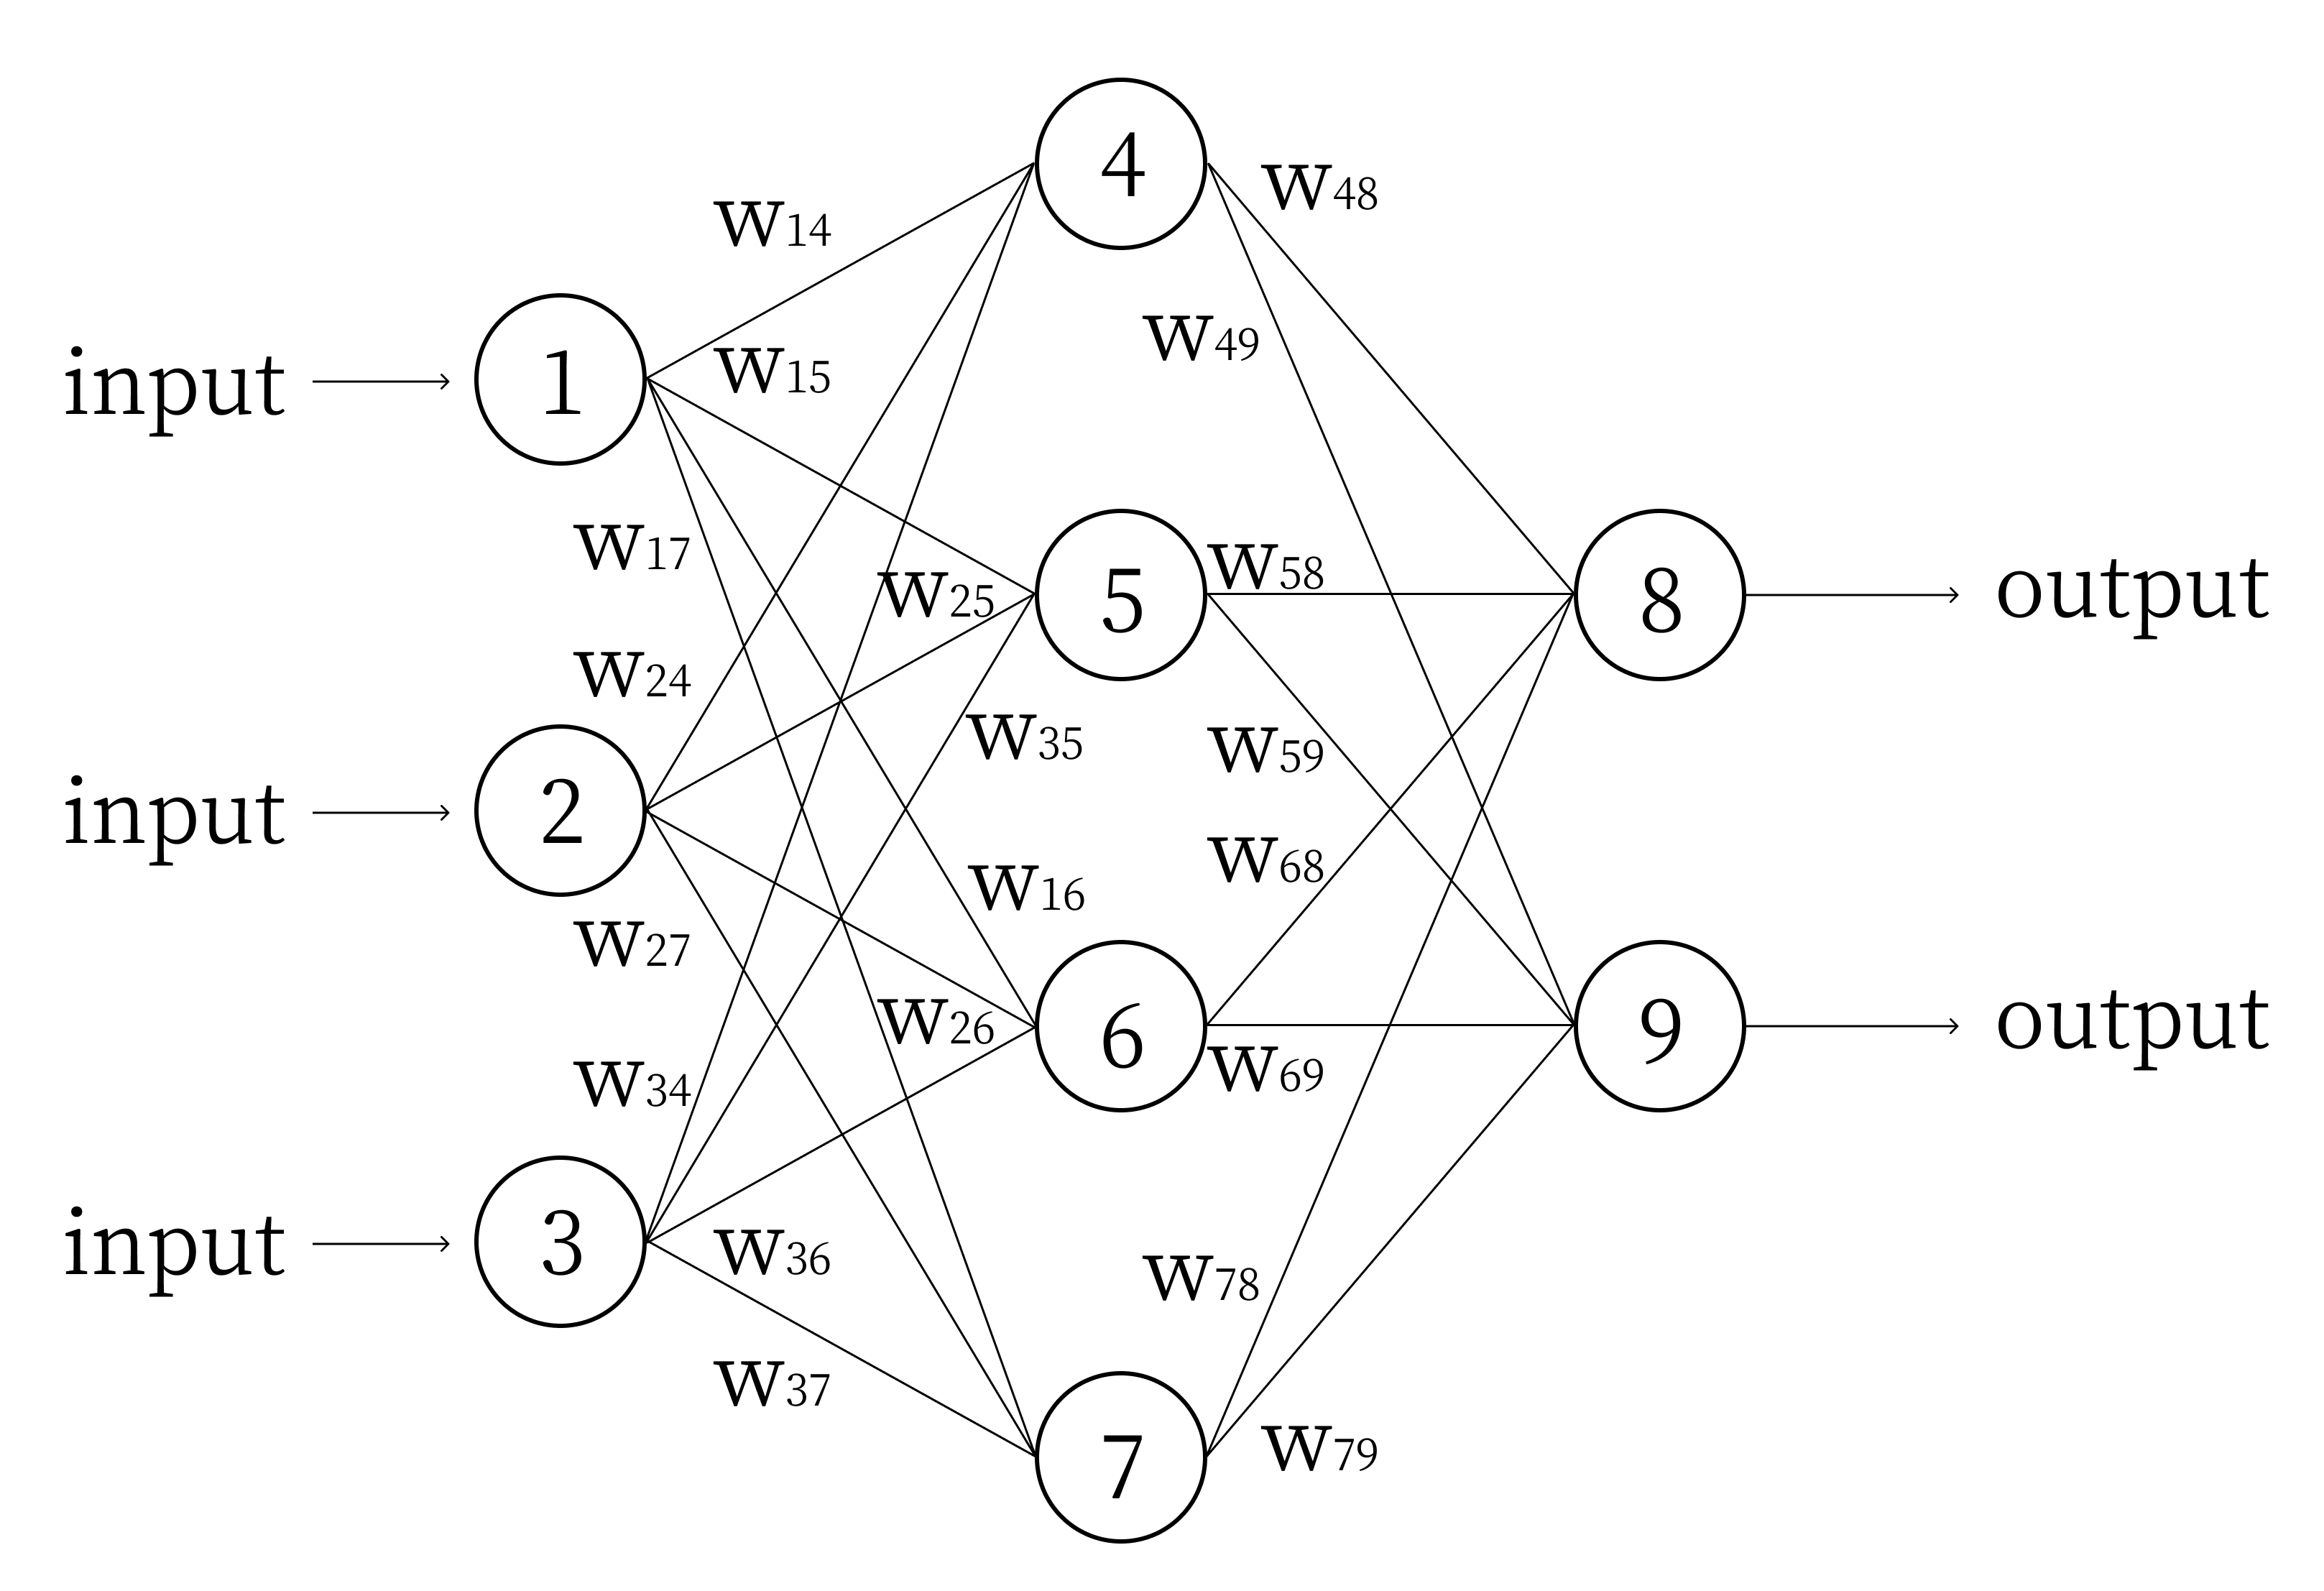
\includegraphics[scale=0.3]{nn2}
\end{center}

Let’s take the partial derivative of the error with respect to a particular weight. Our target outputs are $y_1$ and $y_2$. We define the value at each node $i$ to be $n_i$. We define the bias of node $i$ to be $b_i$. Note that input nodes do not have biases, they are simply input values into the network. We can thus rewrite the error function as:

\[E=\frac{1}{2}\left((n_8-y_1)^2 + (n_9-y_2)^2\right)\]

\subsection{A Simple Example}

Let's calculate $\dfrac{\partial E}{\partial w_{48}}$. By the chain rule:
\[\dfrac{\partial E}{\partial w_{48}} = (n_8-y_1)\left(\frac{\partial{(n_8-y_1)}}{\partial w_{48}}\right)+(n_9-y_2)\left(\frac{\partial{(n_9-y_2)}}{\partial w_{48}}\right)\]

We know:
\[n_8 = \sigma(w_{48}n_4 + w_{58}n_5 + w_{68}n_6 + w_{78}n_7 + b_8).\]
\[n_9 = \sigma(w_{49}n_4 + w_{59}n_5 + w_{69}n_6 + w_{79}n_7 + b_9).\]

Neither $n_9$ nor $y_2$, a part of the target output, depend on $w_{48}$, so the equation becomes:

\[\dfrac{\partial E}{\partial w_{48}} = (n_8-y_1)\left(\frac{\partial{(n_8-y_1)}}{\partial w_{48}}\right)\]

Let's look at $\dfrac{\partial{(n_8-y_1)}}{\partial w_{48}}$. $y_1$ does not depend on $w_{48}$. Looking at $n_8$, we see that the only term in the sigmoid function that depends on $w_{48}$ is $w_{48}n_4$. Thus:
\[\frac{\partial{(n_8-y_1)}}{\partial w_{48}} = \frac{\partial{(\sigma(w_{48}n_4 + w_{58}n_5 + w_{68}n_6 + w_{78}n_7 + b_8))}}{\partial w_{48}}\]
\[\frac{\partial{(n_8-y_1)}}{\partial w_{48}} = \sigma'(w_{48}n_4 + w_{58}n_5 + w_{68}n_6 + w_{78}n_7 + b_8)\frac{\partial{w_{48}n_4}}{\partial w_{48}}\]

We know:
\[n_4 = \sigma(w_{14}n_1 + w_{24}n_2 + w_{34}n_3 + b_4).\]

This equation does not involve $w_{48}$. So we get:

\[\frac{\partial{(n_8-y_1)}}{\partial w_{48}} = \sigma'(w_{48}n_4 + w_{58}n_5 + w_{68}n_6 + w_{78}n_7 + b_8)n_4\]

Substituting back in, we finally arrive at:

\[\dfrac{\partial E}{\partial w_{48}} = (n_8-y_1)\sigma'(w_{48}n_4 + w_{58}n_5 + w_{68}n_6 + w_{78}n_7 + b_8)n_4\]

To shorten this expression, we'll refer to $\sigma'(w_{48}n_4 + w_{58}n_5 + w_{68}n_6 + w_{78}n_7 + b_8)$ as $\sigma_8'$.
\[\dfrac{\partial E}{\partial w_{48}} = (n_8-y_1)\sigma_8'n_4\]

\subsection{Updating Weights}
A network learns by changing its weights to minimize the error. Now that we've figured out the partial derivative of $$w_{48}$$ with respect to the error, we simply update $$w_{48}$$ according to the following rule:

\[w_{48} = w_{48} - \alpha\dfrac{\partial E}{\partial w_{48}}\]

Where $\alpha$ is the learning rate, or some constant.

\subsection{A Complex Example}
Let's begin calculating $\dfrac{\partial E}{\partial w_{14}}$. We know that $y_1$ and $y_2$ are just constants. We also know

\[n_8 = \sigma(w_{48}n_4 + w_{58}n_5 + w_{68}n_6 + w_{78}n_7 + b_8)\]
\[n_9 = \sigma(w_{49}n_4 + w_{59}n_5 + w_{69}n_6 + w_{79}n_7 + b_9)\]
\[n_4 = \sigma(w_{14}n_1 + w_{24}n_2 + w_{34}n_3 + b_4)\]

Nowhere else does $w_{14}$ appear in the network. Let's begin chain-ruling.

\[\dfrac{\partial E}{\partial w_{14}} = (n_8-y_1)\left(\frac{\partial{(n_8-y_1)}}{\partial w_{14}}\right)+(n_9-y_2)\left(\frac{\partial{(n_9-y_2)}}{\partial w_{14}}\right)\]

\subsubsection{Calculations}

The process for calculating each of these partial derivatives is extraordinarily similar. Let's just focus on the first part, or:

\[\dfrac{\partial E}{\partial w_{14}} = (n_8-y_1)\left(\frac{\partial{(n_8-y_1)}}{\partial w_{14}}\right)\]
At the end, repeat the following process for the second partial.


\[\dfrac{\partial E}{\partial w_{14}} = (n_8-y_1)\frac{\partial{n_8}}{\partial w_{14}}\]
\[\dfrac{\partial E}{\partial w_{14}} = (n_8-y_1)\frac{\partial{(\sigma(w_{48}n_4 + w_{58}n_5 + w_{68}n_6 + w_{78}n_7 + b_8))}}{\partial w_{14}}\]
\[\dfrac{\partial E}{\partial w_{14}} = (n_8-y_1)\left(\sigma'(w_{48}n_4 + w_{58}n_5 + w_{68}n_6 + w_{78}n_7 + b_8)\right)\frac{\partial{(w_{48}n_4 + w_{58}n_5 + w_{68}n_6 + w_{78}n_7 + b_8)}}{\partial w_{14}}\]

To make our expression shorter, lets just write
\[\sigma'(w_{48}n_4 + w_{58}n_5 + w_{68}n_6 + w_{78}n_7 + b_8)\]
as $\sigma_8'$. We can rewrite what we have so far as:
\[\dfrac{\partial E}{\partial w_{14}} = (n_8-y_1)\sigma_8'\frac{\partial{(w_{48}n_4 + w_{58}n_5 + w_{68}n_6 + w_{78}n_7 + b_8)}}{\partial w_{14}}\]
Let's continue. Remember, only $n_4$ is dependent on $w_{14}$.

\[\dfrac{\partial E}{\partial w_{14}} = (n_8-y_1)\sigma_8'\frac{\partial{w_{48}n_4}}{\partial w_{14}}\]
\[\dfrac{\partial E}{\partial w_{14}} = (n_8-y_1)\sigma_8'w_{48}\frac{\partial{(\sigma(w_{14}n_1 + w_{24}n_2 + w_{34}n_3 + b_4))}}{\partial w_{14}}\]
\[\dfrac{\partial E}{\partial w_{14}} = (n_8-y_1)\sigma_8'w_{48}(\sigma'(w_{14}n_1 + w_{24}n_2 + w_{34}n_3 + b_4))\frac{\partial{(w_{14}n_1 + w_{24}n_2 + w_{34}n_3 +b_4)}}{\partial w_{14}}\]

Again, lets just write
\[\sigma'(w_{14}n_1 + w_{24}n_2 + w_{34}n_3 + b_4)\]
as $\sigma_4'$. We can rewrite what we have so far as:

\[\dfrac{\partial E}{\partial w_{14}} = (n_8-y_1)\sigma_8'w_{48}\sigma_4'\frac{\partial{(w_{14}n_1 + w_{24}n_2 + w_{34}n_3 + b_4)}}{\partial w_{14}}\]
\[\dfrac{\partial E}{\partial w_{14}} = (n_8-y_1)\sigma_8'w_{48}\sigma_4'\frac{\partial{w_{14}n_1}}{\partial w_{14}}\]
\[\dfrac{\partial E}{\partial w_{14}} = (n_8-y_1)\sigma_8'w_{48}\sigma_4'n_1\]

\subsubsection{The Final Expression}

Let's add back in the second partial. Repeating the calculations, we finally achieve:
\[\dfrac{\partial E}{\partial w_{14}} = (n_8-y_1)\sigma_8'w_{48}\sigma_4'n_1 + (n_9-y_2)\sigma_9'w_{49}\sigma_4'n_1\]
\[\dfrac{\partial E}{\partial w_{14}} = \left((n_8-y_1)\sigma_8'w_{48} + (n_9-y_2)\sigma_9'w_{49}\right)\sigma_4'n_1\]

Of course, in these equations,
\[\sigma_9' = \sigma'(w_{49}n_4 + w_{59}n_5 + w_{69}n_6 + w_{79}n_7 + b_9)\]

\subsection{Biases}
Let's calculate the partial derivative of the error with respect to $b_4$.
As with the weights, let's start chain ruling:
\[\dfrac{\partial E}{\partial b_4} = (n_8-y_1)\left(\frac{\partial{(n_8-y_1)}}{\partial b_4}\right)+(n_9-y_2)\left(\frac{\partial{(n_9-y_2)}}{\partial b_4}\right)\]

Recall that:
\[n_8 = \sigma(w_{48}n_4 + w_{58}n_5 + w_{68}n_6 + w_{78}n_7 + b_8)\]
\[n_9 = \sigma(w_{49}n_4 + w_{59}n_5 + w_{69}n_6 + w_{79}n_7 + b_9)\]
\[n_4 = \sigma(w_{14}n_1 + w_{24}n_2 + w_{34}n_3 + b_4)\]

Let's look at $\frac{\partial{(n_8-y_1)}}{\partial b_4}$. Looking at $n_8$, we see that the only term in the sigmoid function that relies on $b_4$ is $w_{48}n_4$, and $w_{48}$ is constant with respect to $b_4$. Armed with this knowledge, we start chain-ruling:

\[\frac{\partial{(n_8-y_1)}}{\partial b_4} =  \sigma'(w_{48}n_4 + w_{58}n_5 + w_{68}n_6 + w_{78}n_7 + b_8)(w_{48})\frac{\partial{n_4}}{\partial b_4} \]

Let's break down $\frac{\partial{n_4}}{\partial b_4}$. Looking at $n_4$, we see that the only term inside the sigmoid function that relies on $b_4$ is $b_4$ itself, whose derivative is just $1$. Thus:

\[\frac{\partial{n_4}}{\partial b_4} = \sigma'(w_{14}n_1 + w_{24}n_2 + w_{34}n_3 + b_4) \]

Substituting and using our previous shorthand notation, we find:
\[\frac{\partial{(n_8-y_1)}}{\partial b_4} =  (\sigma_8')(\sigma_4')(w_{48})\]

We can use the same process to find that:
\[\frac{\partial{(n_9-y_2)}}{\partial b_4} = (\sigma_9')(\sigma_4')(w_{49}) \]

Finally, we get:
\[\dfrac{\partial E}{\partial b_4} = \sigma_4'((n_8-y_1)\sigma_8'w_{48} + (n_9-y_2)\sigma_9'w_{49})\]

The process is simpler for the third layer.
Take $b_8$ for example. We start the same way:
\[\dfrac{\partial E}{\partial b_8} = (n_8-y_1)\left(\frac{\partial{(n_8-y_1)}}{\partial b_8}\right)+(n_9-y_2)\left(\frac{\partial{(n_9-y_2)}}{\partial b_8}\right)\]

$n_9$ does not depend on $b_8$, so the right side of the expression evaluates to 0 and goes away. For the left side, again, $y_1$ is constant, so we find that:
\[\dfrac{\partial E}{\partial b_8} = (n_8-y_1)\frac{\partial{n_8}}{\partial b_8}\]
The only term in the sigmoid function in the expression for $n_8$ is $b_8$ itself. Thus:
\[\dfrac{\partial E}{\partial b_8} = (n_8-y_1)\sigma_8'\]

\section{A Matrix Representation}
%TODO: Derive the Matrix expressions in "Neural Networks: Part 2", Section 4.5 from the partial derivatives calculated in the non-vectorized fashion.
%Do so for both weight matrices, then the bias matrices. Then provide the general-form equations, which are hopefully self-explanatory by that point.
Let's first define the vectorized network (we've done this in "Neural Networks: Part 2" already). In this case:

\[W_1 =
\begin{bmatrix}
    w_{14} && w_{24} && w_{34} \\
    w_{15} && w_{25} && w_{35} \\
    w_{16} && w_{36} && w_{36} \\
    w_{17} && w_{27} && w_{37} \\
\end{bmatrix}
\qquad
W_2 =
\begin{bmatrix}
    w_{48} && w_{58} && w_{68} && w_{78}\\
    w_{49} && w_{59} && w_{69} && w_{79}\\
\end{bmatrix}
\]
\[x_0 =
\begin{bmatrix}
    n_1 \\
    n_2 \\
    n_3 \\
\end{bmatrix}
\qquad
x_1 =
\begin{bmatrix}
    n_4 \\
    n_5 \\
    n_6 \\
    n_7 \\
\end{bmatrix}
\qquad
x_2 =
\begin{bmatrix}
    n_8 \\
    n_9 \\
\end{bmatrix}
\]
\[
b_1 =
\begin{bmatrix}
    b_4 \\
    b_5 \\
    b_6 \\
    b_7 \\
\end{bmatrix}
\qquad
b_2 =
\begin{bmatrix}
    b_8 \\
    b_9 \\
\end{bmatrix}
\qquad
y =
\begin{bmatrix}
    y_1 \\
    y_2 \\
\end{bmatrix}
\]

And from vectorized forward propagation, we know
\[x_1 = \sigma(W_1x_0 + b_1)\]
\[x_2 = \sigma(W_2x_1 + b_2)\]

Note that

\[W_1x_0 =
\begin{bmatrix}
    w_{14} && w_{24} && w_{34} \\
    w_{15} && w_{25} && w_{35} \\
    w_{16} && w_{36} && w_{36} \\
    w_{17} && w_{27} && w_{37} \\
\end{bmatrix}
\begin{bmatrix}
    n_1 \\
    n_2 \\
    n_3 \\
\end{bmatrix}
=
\begin{bmatrix}
    w_{14}n_1 + w_{24}n_2 + w_{34}n_3 + b_4 \\
    w_{15}n_1 + w_{25}n_2 + w_{35}n_3 + b_5 \\
    w_{16}n_1 + w_{26}n_2 + w_{36}n_3 + b_6 \\
    w_{17}n_1 + w_{27}n_2 + w_{37}n_3 + b_7 \\
\end{bmatrix}
\]

\[W_2x_1 =
\begin{bmatrix}
    w_{48} && w_{58} && w_{68} && w_{78}\\
    w_{49} && w_{59} && w_{69} && w_{79}\\
\end{bmatrix}
\begin{bmatrix}
    n_4 \\
    n_5 \\
    n_6 \\
    n_7 \\
\end{bmatrix}
=
\begin{bmatrix}
    w_{48}n_4 + w_{58}n_5 + w_{68}n_6 + w_{78}n_7 + b_8 \\
    w_{49}n_4 + w_{59}n_5 + w_{69}n_6 + w_{79}n_7 + b_9 \\
\end{bmatrix}
\]
\subsection{The First Matrix}

We can repeat the process outlined in Section 2.2 to calculate the partial derivative of the error function with respect to each weight. The final results for the weights between the second and third layers of nodes follow a similar pattern:

\begin{center}
\qquad $\dfrac{\partial E}{\partial w_{48}} = (n_8-y_1)\sigma_8'n_4$
\qquad $\dfrac{\partial E}{\partial w_{49}} = (n_9-y_2)\sigma_9'n_4$

\end{center}

\begin{center}
\qquad $\dfrac{\partial E}{\partial w_{58}} = (n_8-y_1)\sigma_8'n_5$
\qquad $\dfrac{\partial E}{\partial w_{59}} = (n_9-y_2)\sigma_9'n_5$
\end{center}

\begin{center}
\qquad $\dfrac{\partial E}{\partial w_{68}} = (n_8-y_1)\sigma_8'n_6$
\qquad $\dfrac{\partial E}{\partial w_{69}} = (n_9-y_2)\sigma_9'n_6$
\end{center}

\begin{center}
\qquad $\dfrac{\partial E}{\partial w_{78}} = (n_8-y_1)\sigma_8'n_7$
\qquad $\dfrac{\partial E}{\partial w_{79}} = (n_9-y_2)\sigma_9'n_7$
\end{center}


Hmmmm... these all look similar! I bet we could rearrange them to create a more compact matrix representation, which we will call $\frac{\partial E}{\partial W_2}$. We wish to simplify weight updating to just

\[W_2 = W_2 - \alpha\dfrac{\partial E}{\partial W_2}\]
So, $\dfrac{\partial E}{\partial W_2}$ must be the same shape as $W_2$, which is $2 \times 4$.
\renewcommand{\arraystretch}{2.5}
\[
\dfrac{\partial E}{\partial W_2} =
\begin{bmatrix}
    \dfrac{\partial E}{\partial w_{48}} && \dfrac{\partial E}{\partial w_{58}}  && \dfrac{\partial E}{\partial w_{68}}  && \dfrac{\partial E}{\partial w_{78}} \\
    \dfrac{\partial E}{\partial w_{49}} && \dfrac{\partial E}{\partial w_{59}}  && \dfrac{\partial E}{\partial w_{69}}  && \dfrac{\partial E}{\partial w_{79}} \\
\end{bmatrix}
\]
\renewcommand{\arraystretch}{1}

Note that:
\[
\begin{bmatrix}
    (n_8-y_1)\sigma_8' \\
    (n_9-y_2)\sigma_9' \\
\end{bmatrix}
\begin{bmatrix}
    n_4 && n_5 && n_6 && n_7 \\
\end{bmatrix}
=
\renewcommand{\arraystretch}{2.5}
\begin{bmatrix}
    \dfrac{\partial E}{\partial w_{48}} && \dfrac{\partial E}{\partial w_{58}}  && \dfrac{\partial E}{\partial w_{68}}  && \dfrac{\partial E}{\partial w_{78}} \\
    \dfrac{\partial E}{\partial w_{49}} && \dfrac{\partial E}{\partial w_{59}}  && \dfrac{\partial E}{\partial w_{69}}  && \dfrac{\partial E}{\partial w_{79}} \\
\end{bmatrix}
\]
\renewcommand{\arraystretch}{1}
We can also write this as:
\[
\begin{bmatrix}
    n_8-y_1 \\
    n_9-y_2 \\
\end{bmatrix}
\odot
\begin{bmatrix}
    \sigma_8' \\
    \sigma_9' \\
\end{bmatrix}
\begin{bmatrix}
    n_4 && n_5 && n_6 && n_7 \\
\end{bmatrix}
=
\renewcommand{\arraystretch}{2.5}
\begin{bmatrix}
    \dfrac{\partial E}{\partial w_{48}} && \dfrac{\partial E}{\partial w_{58}}  && \dfrac{\partial E}{\partial w_{68}}  && \dfrac{\partial E}{\partial w_{78}} \\
    \dfrac{\partial E}{\partial w_{49}} && \dfrac{\partial E}{\partial w_{59}}  && \dfrac{\partial E}{\partial w_{69}}  && \dfrac{\partial E}{\partial w_{79}} \\
\end{bmatrix}
\]
Where $\odot$ is the Hadamard product, or element-wise multiplication. Let's vectorize this more:
\[
\begin{bmatrix}
    \sigma_8' \\
    \sigma_9' \\
\end{bmatrix}
=
\begin{bmatrix}
    \sigma'(w_{48}n_4 + w_{58}n_5 + w_{68}n_6 + w_{78}n_7 + b_9) \\
    \sigma'(w_{49}n_4 + w_{59}n_5 + w_{69}n_6 + w_{79}n_7 + b_9) \\
\end{bmatrix}
=
\sigma'(W_2x_1)
\]
\[
\begin{bmatrix}
    n_8-y_1 \\
    n_9-y_2 \\
\end{bmatrix}
=
\begin{bmatrix}
    n_8 \\
    n_9 \\
\end{bmatrix}
-
\begin{bmatrix}
    y_1 \\
    y_2 \\
\end{bmatrix}
=
x_2-y
\]
\[
\begin{bmatrix}
    n_4 && n_5 && n_6 && n_7 \\
\end{bmatrix}
=
x_1^T
\]

Thus, we get
\[\dfrac{\partial E}{\partial W_2} = [(x_2 - y) \odot \sigma'(W_2x_1)]x_1^T\]

For the sake of simplicity, we define
\[\delta_2 = (x_2 - y) \odot \sigma'(W_2x_1)\]

Finally, we reach our old vectorized backpropagation formula:
\[\dfrac{\partial E}{\partial W_2} = \delta_2x_1^T\]

\subsection{The Second Matrix}
We can repeat the process outlined in Section 2.4 to calculate the partial derivative of the error function with respect to each weight. The final results for the weights between the first and second layers of nodes follow a similar pattern:

\[\dfrac{\partial E}{\partial w_{14}} =  \left((n_8-y_1)\sigma_8'w_{48} + (n_9-y_2)\sigma_9'w_{49}\right)\sigma_4'n_1\]
\[\dfrac{\partial E}{\partial w_{15}} =  \left((n_8-y_1)\sigma_8'w_{58} + (n_9-y_2)\sigma_9'w_{59}\right)\sigma_5'n_1\]
\[\dfrac{\partial E}{\partial w_{16}} =  \left((n_8-y_1)\sigma_8'w_{68} + (n_9-y_2)\sigma_9'w_{69}\right)\sigma_6'n_1\]
\[\dfrac{\partial E}{\partial w_{17}} =  \left((n_8-y_1)\sigma_8'w_{78} + (n_9-y_2)\sigma_9'w_{79}\right)\sigma_7'n_1\]
\[\dfrac{\partial E}{\partial w_{24}} =  \left((n_8-y_1)\sigma_8'w_{48} + (n_9-y_2)\sigma_9'w_{49}\right)\sigma_4'n_2\]
\[\dfrac{\partial E}{\partial w_{25}} =  \left((n_8-y_1)\sigma_8'w_{58} + (n_9-y_2)\sigma_9'w_{59}\right)\sigma_5'n_2\]
\[\dfrac{\partial E}{\partial w_{26}} =  \left((n_8-y_1)\sigma_8'w_{68} + (n_9-y_2)\sigma_9'w_{69}\right)\sigma_6'n_2\]
\[\dfrac{\partial E}{\partial w_{27}} =  \left((n_8-y_1)\sigma_8'w_{78} + (n_9-y_2)\sigma_9'w_{79}\right)\sigma_7'n_2\]
\[\dfrac{\partial E}{\partial w_{34}} =  \left((n_8-y_1)\sigma_8'w_{48} + (n_9-y_2)\sigma_9'w_{49}\right)\sigma_4'n_3\]
\[\dfrac{\partial E}{\partial w_{35}} =  \left((n_8-y_1)\sigma_8'w_{58} + (n_9-y_2)\sigma_9'w_{59}\right)\sigma_5'n_3\]
\[\dfrac{\partial E}{\partial w_{36}} =  \left((n_8-y_1)\sigma_8'w_{68} + (n_9-y_2)\sigma_9'w_{69}\right)\sigma_6'n_3\]
\[\dfrac{\partial E}{\partial w_{37}} =  \left((n_8-y_1)\sigma_8'w_{78} + (n_9-y_2)\sigma_9'w_{79}\right)\sigma_7'n_3\]

To update each respective weight, we would subtract these partials (multiplied by $\alpha$) from their respective weights, just as we did for $w_{14}$ above.

Our matrix representation needs to look like this:

\renewcommand{\arraystretch}{2.5}
\[
\dfrac{\partial E}{\partial W_1} =
\begin{bmatrix}
    \dfrac{\partial E}{\partial w_{14}} && \dfrac{\partial E}{\partial w_{24}}  && \dfrac{\partial E}{\partial w_{34}}  \\
    \dfrac{\partial E}{\partial w_{15}} && \dfrac{\partial E}{\partial w_{25}}  && \dfrac{\partial E}{\partial w_{35}}  \\
    \dfrac{\partial E}{\partial w_{16}} && \dfrac{\partial E}{\partial w_{26}}  && \dfrac{\partial E}{\partial w_{36}}  \\
    \dfrac{\partial E}{\partial w_{17}} && \dfrac{\partial E}{\partial w_{27}}  && \dfrac{\partial E}{\partial w_{37}}  \\
\end{bmatrix}
\]
\renewcommand{\arraystretch}{1}

We notice that:
\[
\begin{bmatrix}
    w_{48} & w_{49} \\
    w_{58} & w_{59} \\
    w_{68} & w_{69} \\
    w_{78} & w_{79}
\end{bmatrix}
\begin{bmatrix}
    \sigma_8'n_8-y_1 \\
    \sigma_9'n_9-y_2
\end{bmatrix}
=
\begin{bmatrix}
    w_{48}\sigma_8'(n_8-y_1) + w_{49}\sigma_9'(n_9-y_2) \\
    w_{58}\sigma_8'(n_8-y_1) + w_{59}\sigma_9'(n_9-y_2) \\
    w_{68}\sigma_8'(n_8-y_1) + w_{69}\sigma_9'(n_9-y_2) \\
    w_{78}\sigma_8'(n_8-y_1) + w_{79}\sigma_9'(n_9-y_2) \\
\end{bmatrix}
\]
Which can be vectorized and simplified as:
\[
\begin{bmatrix}
    w_{48} & w_{49} \\
    w_{58} & w_{59} \\
    w_{68} & w_{69} \\
    w_{78} & w_{79}
\end{bmatrix}
\left(
\begin{bmatrix}
    \sigma_8' \\
    \sigma_9'
\end{bmatrix}
\odot
\begin{bmatrix}
    n_8-y_1 \\
    n_9-y_2
\end{bmatrix}
\right)
=
\begin{bmatrix}
    w_{48}\sigma_8'(n_8-y_1) + w_{49}\sigma_9'(n_9-y_2) \\
    w_{58}\sigma_8'(n_8-y_1) + w_{59}\sigma_9'(n_9-y_2) \\
    w_{68}\sigma_8'(n_8-y_1) + w_{69}\sigma_9'(n_9-y_2) \\
    w_{78}\sigma_8'(n_8-y_1) + w_{79}\sigma_9'(n_9-y_2) \\
\end{bmatrix}
\]
\[
W_2^T[\sigma'(W_2x_1) \odot (x_2-y)] =
\begin{bmatrix}
    w_{48}\sigma_8'(n_8-y_1) + w_{49}\sigma_9'(n_9-y_2) \\
    w_{58}\sigma_8'(n_8-y_1) + w_{59}\sigma_9'(n_9-y_2) \\
    w_{68}\sigma_8'(n_8-y_1) + w_{69}\sigma_9'(n_9-y_2) \\
    w_{78}\sigma_8'(n_8-y_1) + w_{79}\sigma_9'(n_9-y_2) \\
\end{bmatrix}
\]
\[
W_2^T\delta_2 =
\begin{bmatrix}
    w_{48}\sigma_8'(n_8-y_1) + w_{49}\sigma_9'(n_9-y_2) \\
    w_{58}\sigma_8'(n_8-y_1) + w_{59}\sigma_9'(n_9-y_2) \\
    w_{68}\sigma_8'(n_8-y_1) + w_{69}\sigma_9'(n_9-y_2) \\
    w_{78}\sigma_8'(n_8-y_1) + w_{79}\sigma_9'(n_9-y_2) \\
\end{bmatrix}
\]

This $\delta_2$ is the same as the one we defined when calculating the previous vectorized representation. Now, this is fine and dandy, but we've so far ignored the $\sigma_4'n_1$ and the $\sigma_5'n_1$ etc. sitting outside the parends of our partial derivative calculation. Let's work those in.
\[
\left(
\begin{bmatrix}
    w_{48}\sigma_8'(n_8-y_1) + w_{49}\sigma_9'(n_9-y_2) \\
    w_{58}\sigma_8'(n_8-y_1) + w_{59}\sigma_9'(n_9-y_2) \\
    w_{68}\sigma_8'(n_8-y_1) + w_{69}\sigma_9'(n_9-y_2) \\
    w_{78}\sigma_8'(n_8-y_1) + w_{79}\sigma_9'(n_9-y_2) \\
\end{bmatrix}
\odot
\begin{bmatrix}
    \sigma_4' \\
    \sigma_5' \\
    \sigma_6' \\
    \sigma_7' \\
\end{bmatrix}
\right)
\begin{bmatrix}
    n_1 && n_2 && n_3
\end{bmatrix}
=
\]
\[
\begin{bmatrix}
    \left((n_8-y_1)\sigma_8'w_{48} + (n_9-y_2)\sigma_9'w_{49}\right)\sigma_4'n_1 && \left((n_8-y_1)\sigma_8'w_{48} + (n_9-y_2)\sigma_9'w_{49}\right)\sigma_4'n_2  && \left((n_8-y_1)\sigma_8'w_{48} + (n_9-y_2)\sigma_9'w_{49}\right)\sigma_4'n_3  \\
     \left((n_8-y_1)\sigma_8'w_{58} + (n_9-y_2)\sigma_9'w_{59}\right)\sigma_5'n_1 && \left((n_8-y_1)\sigma_8'w_{58} + (n_9-y_2)\sigma_9'w_{59}\right)\sigma_5'n_2  &&  \left((n_8-y_1)\sigma_8'w_{58} + (n_9-y_2)\sigma_9'w_{59}\right)\sigma_5'n_3  \\
    \left((n_8-y_1)\sigma_8'w_{68} + (n_9-y_2)\sigma_9'w_{69}\right)\sigma_6'n_1 && \left((n_8-y_1)\sigma_8'w_{68} + (n_9-y_2)\sigma_9'w_{69}\right)\sigma_6'n_2  &&  \left((n_8-y_1)\sigma_8'w_{68} + (n_9-y_2)\sigma_9'w_{69}\right)\sigma_6'n_3  \\
     \left((n_8-y_1)\sigma_8'w_{78} + (n_9-y_2)\sigma_9'w_{79}\right)\sigma_7'n_1 && \left((n_8-y_1)\sigma_8'w_{78} + (n_9-y_2)\sigma_9'w_{79}\right)\sigma_7'n_2  &&  \left((n_8-y_1)\sigma_8'w_{78} + (n_9-y_2)\sigma_9'w_{79}\right)\sigma_7'n_3  \\
\]
\[
=
\renewcommand{\arraystretch}{2.5}
\begin{bmatrix}
    \dfrac{\partial E}{\partial w_{14}} && \dfrac{\partial E}{\partial w_{24}}  && \dfrac{\partial E}{\partial w_{34}}  \\
    \dfrac{\partial E}{\partial w_{15}} && \dfrac{\partial E}{\partial w_{25}}  && \dfrac{\partial E}{\partial w_{35}}  \\
    \dfrac{\partial E}{\partial w_{16}} && \dfrac{\partial E}{\partial w_{26}}  && \dfrac{\partial E}{\partial w_{36}}  \\
    \dfrac{\partial E}{\partial w_{17}} && \dfrac{\partial E}{\partial w_{27}}  && \dfrac{\partial E}{\partial w_{37}}  \\
\end{bmatrix}
\renewcommand{\arraystretch}{1}
=
\dfrac{\partial E}{\partial W_1}
\]

Note that
\[
\begin{bmatrix}
    \sigma_4' \\
    \sigma_5' \\
    \sigma_6' \\
    \sigma_7' \\
\end{bmatrix}
 =
 \sigma'\left(
 \begin{bmatrix}
     w_{14}n_1 + w_{24}n_2 + w_{34}n_3 + b_4 \\
     w_{15}n_1 + w_{25}n_2 + w_{35}n_3 + b_5 \\
     w_{16}n_1 + w_{26}n_2 + w_{36}n_3 + b_6 \\
     w_{17}n_1 + w_{27}n_2 + w_{37}n_3 + b_7 \\
 \end{bmatrix}
 \right)
 =
 \sigma'(W_1x_0)
 \]
 \[ x_0^T = \begin{bmatrix}
    n_1 && n_2 && n_3
\end{bmatrix}
\]

Thus, we get
\[
\dfrac{\partial E}{\partial W_1} =
[W_2^T\delta_2 \odot \sigma'(W_1x_0)]x_0^T
\]

We denote
\[\delta_1 = W_2^T\delta_2 \odot \sigma'(W_1x_0)\]
yielding
\[\dfrac{\partial E}{\partial W_1} = \delta_1x_0^T\]


\subsection{The Bias Vectors}
For the second layer, the biases are:
\[\dfrac{\partial E}{\partial b_4} = \sigma_4'((n_8-y_1)\sigma_8'w_{48} + (n_9-y_2)\sigma_9'w_{49})\]
\[\dfrac{\partial E}{\partial b_5} = \sigma_5'((n_8-y_1)\sigma_8'w_{58} + (n_9-y_2)\sigma_9'w_{59})\]
\[\dfrac{\partial E}{\partial b_6} = \sigma_6'((n_8-y_1)\sigma_8'w_{68} + (n_9-y_2)\sigma_9'w_{69})\]
\[\dfrac{\partial E}{\partial b_7} = \sigma_7'((n_8-y_1)\sigma_8'w_{78} + (n_9-y_2)\sigma_9'w_{79})\]
For the third layer, the biases are:
\[\dfrac{\partial E}{\partial b_8} = (n_8-y_1)\sigma_8'\]
\[\dfrac{\partial E}{\partial b_9} = (n_9-y_2)\sigma_9'\]

We wish to have a simple way to express how to update the bias matrix, like so:

\[ b_i = b_i - \alpha\dfrac{\partial E}{\partial b_i}  \]

where $b_i$ is a matrix. In other words, we need to calculate $\dfrac{\partial E}{\partial b_i}$ Let's look at the second layer first. $b_1$ is a 4 x 1 matrix, so $\dfrac{\partial E}{\partial b_1}$ must have the same dimensions. Without vectors, our update is:

\[ b_j = b_j - \alpha\dfrac{\partial E}{\partial b_j}\]

where $b_j$ is the bias for a single node, i.e. an element of a bias matrix. Looking at the partials for the biases of the second layer, we can simply define $b_1$ as the 4 x 1 matrix of each bias like so:

\[
\dfrac{\partial E}{\partial b_1} =
\begin{bmatrix}
    \dfrac{\partial E}{\partial b_4} \\ \\
    \dfrac{\partial E}{\partial b_5} \\ \\
    \dfrac{\partial E}{\partial b_6} \\ \\
    \dfrac{\partial E}{\partial b_7} \\
\end{bmatrix}
\]

Similarly, for the second bias matrix:

\[
\dfrac{\partial E}{\partial b_2} =
\begin{bmatrix}
    \dfrac{\partial E}{\partial b_8} \\ \\
    \dfrac{\partial E}{\partial b_9} \\
\end{bmatrix}
\]
To derive our equations for the bias update for vectorized backpropagation, let's first look at the second bias matrix. If write out each element, we find:
\[
\dfrac{\partial E}{\partial b_2} =
\begin{bmatrix}
    (n_8-y_1)\sigma_8' \\ \\
    (n_9-y_2)\sigma_9' \\
\end{bmatrix}
=
\begin{bmatrix}
    (n_8-y_1)\sigma'(w_{48}n_4 + w_{58}n_5 + w_{68}n_6 + w_{78}n_7 + b_8) \\ \\
    (n_9-y_2)\sigma'(w_{49}n_4 + w_{59}n_5 + w_{69}n_6 + w_{79}n_7 + b_9) \\
\end{bmatrix}
\]
We can rewrite this as a Hadamard product:
\[
\dfrac{\partial E}{\partial b_2} =
\begin{bmatrix}
    n_8-y_1 \\ \\
    n_9-y_2 \\
\end{bmatrix}
\odot
\begin{bmatrix}
    \sigma'(w_{48}n_4 + w_{58}n_5 + w_{68}n_6 + w_{78}n_7 + b_8) \\ \\
    \sigma'(w_{49}n_4 + w_{59}n_5 + w_{69}n_6 + w_{79}n_7 + b_9) \\
\end{bmatrix}
\]
The first matrix can be written in vectorized form as $x_2 - y$, and the second matrix can be written as $\sigma'(W_2x_1)$. We can then arrive at:
\[
\dfrac{\partial E}{\partial b_2} = (x_2 - y) \odot (\sigma'(W_2x_1))
\]
Notice that this is the same as the $\delta_2$ we calculated for the weights earlier. We can write the bias formula as just:
\[\dfrac{\partial E}{\partial b_2} = \delta_2\]


Looking at the first bias matrix, we see that we can write it out as:
\[
\dfrac{\partial E}{\partial b_1} =
\begin{bmatrix}
    \sigma_4'((n_8-y_1)\sigma_8'w_{48} + (n_9-y_2)\sigma_9'w_{49}) \\ \\
    \sigma_5'((n_8-y_1)\sigma_8'w_{58} + (n_9-y_2)\sigma_9'w_{59}) \\ \\
    \sigma_6'((n_8-y_1)\sigma_8'w_{68} + (n_9-y_2)\sigma_9'w_{69}) \\ \\
    \sigma_7'((n_8-y_1)\sigma_8'w_{78} + (n_9-y_2)\sigma_9'w_{79}) \\
\end{bmatrix}
\]
Looking carefully at this matrix, we see that we can write it out as a product of two matrices including $\dfrac{\partial E}{\partial b_2}$.
\[
\dfrac{\partial E}{\partial b_1} =
\begin{bmatrix}
    \sigma'_4w_{48} && \sigma'_4w_{49} \\
    \sigma'_5w_{58} && \sigma'_5w_{59} \\
    \sigma'_6w_{68} && \sigma'_6w_{69} \\
    \sigma'_7w_{78} && \sigma'_7w_{79}
\end{bmatrix}
\begin{bmatrix}
    (n_8-y_1)\sigma_8' \\ \\
    (n_9-y_2)\sigma_9' \\
\end{bmatrix}
\]
The first matrix looks very similar to some combination of $W_2$ and $\sigma'(W_2x_1)$. We can rewrite and rearrange the equation with the help of the Hadamard product:
\[
\dfrac{\partial E}{\partial b_1} =
\begin{bmatrix}
    w_{48} && w_{49} \\
    w_{58} && w_{59} \\
    w_{68} && w_{69} \\
    w_{78} && w_{79}
\end{bmatrix}
\begin{bmatrix}
    (n_8-y_1)\sigma_8' \\ \\
    (n_9-y_2)\sigma_9' \\
\end{bmatrix}
\odot
\begin{bmatrix}
    \sigma'_4 \\
    \sigma'_5 \\
    \sigma'_6 \\
    \sigma'_7
\end{bmatrix}
\]
This, in turn, can be written as
\[
\dfrac{\partial E}{\partial b_1} =
W_2^T\dfrac{\partial E}{\partial b_2} \odot \sigma'(W_2x_1)
\]
\[
\dfrac{\partial E}{\partial b_1} =
W_2^T\delta_2 \odot \sigma'(W_2x_1)
\]

Hey\ldots this is the same as $\delta_1$ from earlier! Now our equation is just:
\[
\dfrac{\partial E}{\partial b_1} = \delta_1
\]

\subsection{A General Form}
We can generalize this for any layer. The only difference is the delta for the last layer:
\[\delta_L = (x_L - y) \odot \sigma'(W_{L}x_{L-1})\]

The delta for every other layer is:
\[\delta_i = W_{i+1}^T\delta_{i+1} \odot \sigma'(W_ix_{i-1})\]

And the gradient for every weight matrix are calculated and the weight matrices are updated as follows:
\[\frac{\partial E}{\partial W_i} = \delta_i x_{i-1}^T\]

\[W_i =  W_i - \alpha \frac{\partial E}{\partial W_i}\]

For biases, the rule is simpler:

\[b_i =  b_i - \alpha \delta_i\]

That is the essence of backpropagation. Note that these formulas work for any activation function. The reason sigmoid is used to teach is because its derivative is fairly straightforward:
\[\sigma'(x) = \sigma(x)(1-\sigma(x))\]
\end{document}
